\chapter{Introduction}
It is now the fiftieth anniversary since the link between the protein amino acid sequence and its three-dimensional structure was celebrated \cite{anfinsen1973principles} by the awarding of a Nobel prize to Anfinsen in 1972 for this important observation \cite{anfinsen1972nobel}.  Anfinsen showed that if a protein is heated it will unravel and fold back to its original state when cooled, demonstrating that a protein's native structure is determined by the properties of the amino acids that it is composed of, rather than the folding being carried out by intracellular machinery.  This insight means that theoretically, a protein's structure can be predicted based on its amino acid sequence.  Until the structure of poorly characterised protein families can be elucidated experimentally, ab initio protein modelling using sequence only can be used to predict a fold allowing for structure-based function inferences \cite{Rigden2017_a,rigden2017prediction,bandyopadhyay2006structure,da2012structure}.  1994 began the biannual CASP (Critical Assessment of Structure Prediction) challenge \cite{jones1999protein} with the objective to advance the computational methods of predicting protein structure from sequence. I have had the fortunate opportunity to be an assessor on the fourteenth and fifteenth CASP competitions \cite{simpkin2021evaluation}.  This PhD thesis focuses on the prediction of specific putative membrane transporter proteins utilising computational approaches to build models and predict their function based on the \textit{ab initio} structure. 

\section{Membrane Proteins}
Lipid membranes form barriers around cells and membrane bound organelles.  These barriers have a thickness of around 35{\AA} and are important for the regulation of molecular traffic across their surface.  The cell membrane's major constituents are amphipathic lipids in the form of phospholipids, glycolipids, and sterols.  Additionally, biological membranes possess  carbohydrates (mostly glycoproteins) and a large content of proteins.  The carbohydrates play an important role in intracellular recognition especially in eukaryotes while membrane proteins have a very diverse array of functions.

Membrane proteins are of considerable medical importance as 30\% of the human genome encodes for membrane proteins \cite{mesdaghi2020silico} and around 50\% of drugs currently on the market target these proteins \cite{overington2006many}.  Membrane proteins can be grouped according to whether they are a permanent fixture of the cell membrane (integral membrane proteins - IMPs) or whether they transiently interact with the cell membrane (peripheral membrane proteins - PMPs).  The temporary association of PMPs with the plasma membrane, either with the lipid bilayer (amphitropic proteins) or an IMP, define this class of membrane proteins. Some proteins such as G-proteins and certain kinases are able interact with both the membrane and a IMP simultaneously \cite{vogler2008membrane}. The association of PMPs with the cell membrane components is a result of non-covalent hydrophobic and electrostatic interactions and therefore dissociate from the membrane in the presence polar reagents.  This transient association with the membrane is important for a variety of cellular processes including cell signalling regulation \cite{cafiso2005structure}, protein-protein interactions \cite{takida2004exocytic} and protein activation through conformational changes \cite{johnson1999amphitropic}.

IMPs on the other hand are permanent fixtures of the cell membrane and are either transmembrane proteins (TMPs) or integral monotopic proteins. TMPs take the form of an $\alpha$-helical structure (or sometimes a $\beta$-barrel in Gram-negative bacteria, chloroplast and mitochondria \cite{selkrig2014assembly}) and cross the full length of the lipid bilayer once (bitopic membrane protein) or multiple times (polytopic transmembrane proteins).  This is in contrast to integral monotopic membrane proteins (or peripheral membrane proteins) which are fixed to one side of the membrane only \cite{baker2017charged}.  As TMPs are very hydrophobic, the residues that cross the membrane forming the membrane spanning segments are mostly hydrophobic and therefore these proteins precipitate in water and it is necessary to use nonpolar solvents or detergents in order to carry out their isolation. Transmembrane regions are more likely to possess secondary structure as the polar backbone carbonyls and amide of the residues form intramolecular hydrogen bonds in a hydrophobic environment thus creating secondary structure. The dielectric environment caused by the polar heads of the phospholipids at the membrane interface region is more likely to hold aromatic residues like tyrosine and tryptophan in addition to the presence of amphipathic $\alpha$-helices \cite{wimley1996solvation}.  

\section{The Function of Membrane Proteins}
Membrane proteins carry out a wide range of essential functions: transport, junctions, enzymes, receptors, signalling (including cell-cell recognition) and anchoring (to the cytoskeleton and extracellular matrix).  The largest family of membrane proteins are the G-protein coupled receptors (which are also the largest family of proteins) and membrane transporter proteins \cite{lesk2021protein}.  The research described in this thesis focuses on the modelling of three distinct integram membrane proteins that are involved in transport. 

Membrane transport proteins control the movements of specific molecules across the cell membrane. Membrane transport proteins are divided into two major groups; channels and transporters.  Channels create an aqueous pore through the membrane bilayer that allow substances to cross the membrane passively down an electrochemical or chemical gradient \cite{alberts2002principles}.  Sometimes the pore is gated and will only open to allow this diffusional process to occur under certain conditions regulating the traffic through the pore.  Transporters on the other hand move specific molecules against their concentration gradients by binding to the substrate and undergoing a series of conformational changes releasing the substrate on the opposite side of the membrane.  The movement of the substrate by a transporter is an active process.  The conformational cycle a transporter undergoes is coupled with ATP hydrolysis or tethered to the presence of ion gradients.  Both sides of the transporter possess a gate that restricts access to the substrate binding site when closed with the alternate confirmations ensuring that only one gate is open at any particular time.  The distinction between channels and transporters is not always clear \cite{ashcroft2009introduction} however.  For example, CLC (Chloride Channel) proteins are a family of membrane transport proteins that mediate the chloride conductance across the cell membrane and were once thought to be exclusively channels.  It is now known that this family also contain transporters that are driven by a proton current in the opposite direction of the flow of chloride ions (proton antiporter).  Indeed, five out of the nine human CLC proteins utilise the antiporter transporter mechanism \cite{miller2009provisional}.  Additionally, palytoxin reversibly converts the ATP hydrolysis coupled Na\textsuperscript{+}/K\textsuperscript{+}-ATPase pump into a non-selective cation channel by rendering both gates to the open position \cite{gadsby2009peering}. 

\section{Challenges of Membrane Protein Structure Determination and Prediction}
A protein’s structural information is crucial to understand its function and evolution. Currently, there is only experimental structural data for a tiny fraction of proteins \cite{Khafizov2014}. For instance, membrane proteins are encoded by 30\% of the protein-coding genes of the human genome \cite{Almen2009}, but they only have a 3.3\% \cite{mesdaghi2020silico}
representation in the Protein Data Bank (PDB) (5785 membrane proteins out of 174507 PDB entries) \cite{mesdaghi2020silico}. Membrane protein families are particularly poorly understood due to experimental difficulties, such as over-expression, which can result in toxicity to host cells \cite{Grisshammer1995}, as well as difficulty in finding a suitable membrane mimetic to reconstitute the protein to allow expression of the native structure.  Membrane proteins are more structured compared to their soluble counterparts as the membrane imposes restraints on the protein \cite{leman2020macromolecular} and this leads to experimental difficulties as membrane mimetics have to be used in order to allow the protein to fold properly.  Membrane mimetics can take the form detergents of lipid.  Detergents possess a single fatty acid chain and form a micelle around the protein which can result in distortions in the protein structure.  Lipids form bicelles around proteins resulting in less chance of protein distortion. Lipids in the form of nanodiscs can also be used where lipid bilayer is contained by amphipathic molecules such as synthetic polymers or peptides \cite{denisov2016nanodiscs}.  A nanodisc is a nanoscale model system. It is a self-assembled lipid bilayer disc stabilized by a belt of membrane scaffold proteins (MSPs). Nanodiscs provide a more native-like environment for studying membrane proteins compared to traditional detergent micelles or liposomes.  The structure of a nanodisc typically consists of a lipid bilayer surrounded by two copies of an amphipathic membrane scaffold protein (MSP) that forms a belt around the rim of the bilayer. The MSPs stabilise the nanodisc by shielding the hydrophobic lipid tails from the surrounding aqueous environment.  Nanodiscs can be reconstituted with specific membrane proteins, allowing their study in a more physiologically relevant lipid environment. The lipid composition of the nanodisc can be customised to mimic the native membrane composition or to modulate the properties of the membrane protein being studied.  The method of protein structure determination as well as the properties of the protein itself  will determine the membrane mimetic to utilise.  Often a screening process is required to identify the most suitable mimetic \cite{bayburt2010membrane}. 

Crystallisation is difficult and may need extensive protein engineering for example insertion of protein FAB (Fragment Antigen-Binding) fragments to allow crystallisation .  The removal of long flexible loops may also be required \cite{rosenbaum2007gpcr}.  Another experimental technique for determining protein structure is NMR (Nuclear Magnetic Resonance). NMR spectroscopy relies on the principles of nuclear magnetic resonance, which involves the interaction between the magnetic properties of atomic nuclei and an external magnetic field.  Further to the difficulties of crystallisation, NMR is difficult as there is a size limit due to protein-detergent tumbling time (rate at which the protein moves). Also, compared to soluble proteins, it is difficult to assign the NMR spectrum to obtain the restraints for the structural data of membrane proteins and calculate  their structure.  NMR relies on nuclear Overhauser enhancement (NOE) restraints that can only be measured at a 5{\AA} threshold which is satisfactory for intrahelical restraints but makes contacts between two helices problematic and therefore fold determination difficult.  NOE restraints are derived from the observation of dipolar interactions between pairs of nuclei in close proximity. These interactions provide valuable distance information that helps in calculating the three-dimensional structure of a protein. However, the efficiency of the NOE effect diminishes as the distance between the interacting nuclei increases. The maximum distance at which NOE interactions can be reliably detected in NMR experiments is typically around 5 {\AA}.  When it comes to interhelical contacts, the distance between the nuclei involved in the NOE restraints can be larger than the 5 {\AA} threshold. Helices within a protein often have specific packing arrangements, and determining the precise contacts between them is crucial for accurately determining the protein's overall fold. However, the limited detection range of NOEs makes it challenging to obtain direct distance restraints for interhelical contacts \cite{vogeli2014nuclear}. The problem can be overcome by identifying side chain assignments in the spectra to measure the restraints but this is also very difficult.  This is the explanation as to why there are more $\beta$-barrel NMR structures compared to $\alpha$-helical as it is much easier to determine the restraints between the strands as they are within the 5{\AA} threshold \cite{kaltschnee2016extraction}. 

Additionally, membrane proteins are much less conserved across species compared to water-soluble proteins \cite{Sojo2016}, making sequence-based homologue identification a challenge, and in turn rendering homology modelling of these proteins more difficult. Sequence similarity and how well the sequences are aligned is positively correlated with homology model accuracy where a similarity of 70\% yields models with RMSDs (Root Mean Square Deviation) under 3{\AA} and RMSDs typically above 3{\AA} for templates with sequence similarities of 25\% \cite{baker2001protein}.  Homology modelling software such as MODELLER \cite{webb2016comparative} takes the alignment and the template to construct a model based of the template by satisfying its spatial constraints obtained from the alignment.  It has been demonstrated that given a high quality alignment and appropriate template MODELLER can construct accurate membrane protein structures \cite{tabassum2014structural}.  For proteins of sequence similarity of less than 25\% threading tools can be used to obtain models.  Threading relies on a multiple sequence alignment of templates which is scored against a knowledge based scoring function including residue pairing.  iTASSER, in conjunction with contact predictions, has been shown to using threading methods to model G-protein coupled receptor membrane proteins and achieve RMSDs of 3{\AA} \cite{yang2015tasser}. 

Molecular dynamics simulations have also been used to fold proteins.  Molecular dynamics (MD) is a computational simulation method used to study the motion and behavior of atoms and molecules over time. 
In MD, the positions, velocities, and forces of atoms or particles are numerically integrated to simulate their dynamic behaviour. The simulations are based on classical mechanics and use interatomic or intermolecular potential energy functions to describe the forces and interactions between particles \cite{hansson2002molecular}.  One of the early successful attempts of protein folding using MD was demonstrated with acylCoA Dehydragenase where a 30ms simulation folded the 80 residue soluble protein \cite{lane2013milliseconds,bonito2016insights}.  Early endeavours to simulate the folding of membrane proteins in a lipid bilayer were fraught with difficulties.  The complex bilayer environment resulted in multi-spanning transmembrane proteins becoming snared in incorrect folds.  The molecular dynamic simulations are very computationally expensive with the number of atomic interactions becoming huge with larger membrane proteins.

Finally, ab initio computational methods for predicting membrane proteins structure is an alternative route to elucidate the structure and function of uncharacterised membrane proteins.  Theoretically, as a result of their smaller conformational search space due to the restraints imposed by the membrane, membrane proteins have an advantage for computational methods of prediction, although the size of membrane proteins are generally larger than their soluble counterparts. Older computational prediction methods such as Rosetta \cite{baker2001protein} struggled with deriving accurate scoring functions as well as molecular force field parameters \cite{koehler2015computational}.  

\section{Secondary Structure and Transmembrane Span Prediction}
Transmembrane region prediction is an important process in the structural characterisation of a membrane protein molecule; both experimentally and computationally.  The presence of hydrophobic patterns in the transmembrane regions of TMPs is used by transmembrane topology prediction software to anticipate the relative positions of transmembrane regions within a given membrane protein sequence \cite{krogh2001predicting}.  Early transmembrane span prediction software used hydrophobicity values from amoving window average and were able to achieve 70\% accuracy \cite{koehler2009unified}.  Various hydrophobicity scales could be utilised which were derived from experimental and predictive methods \cite{koehler2009unified}.  The accuracy to above 90\% was achieved with the introduction of Hidden Markov Models (HMMs), for example TMHMM \cite{krogh2001predicting}, and OCTOPUS which used machine learning to make residue level predictions and HMMs to consolidate the predictions into a global model. OCTOPUS is also trained to predict the presence of re-entrant loops and transmembrane hairpins \cite{viklund2006structural}. With different prediction tools utilising individual algorithms there can be disagreements with the topology predictions and this has given rise to some tools using a consensus method in an attempt to overcome this \cite{Tsirigos2015}. 

The above methods are for the exclusive prediction of transmembrane $\alpha$-helical bundles and obviously cannot identify the presence of $\beta$-barrels. Accurate methods to make $\beta$-barrel predictions utilise both HMMs and machine learning algorithms.  TMbeta-Net \cite{gromiha2005tmbeta} takes the artificial neural network approach while TMBHMM \cite{singh2011tmbhmm} uses HMMs.

Additionally, bioinformatic software is available that predicts the orientation of transmembrane protein models within the membrane bilayer.  The predicted placement of transmembrane protein models within a cell membrane model is not a straightforward task as the membrane possesses uneven polarity gradients as well as a varying molecular organisation.  Both PDBTM \cite{Kozma2012} and OPM \cite{Lomize2012} utilises an algorithm to place proteins structures within membrane boundaries.  Their algorithms minimise the protein's normalised non-polar accessible surface area transfer energy from water to a hydrophobic region acting as an approximation to a cell membrane \cite{Lomize2012,Kozma2012}.

In addition to protein transmembrane span prediction, methods were developed to predict protein secondary structure. The first tools to predict protein secondary structure correlated secondary structure states with single residue statistics, however, their accuracy was not much better than random \cite{rost2000third}.  Subsequently tools were developed that obtained data from larger regions rather than single residues and higher accuracies being obtained when artificial intelligence algorithms (specifically machine learning algorithms)  were introduced.  PSI-PRED, being the most accurate and widely used, utilises a multi layered artificial neural network that takes a position specific scoring matrix to make an initial secondary structure prediction with subsequent layers filtering noise \cite{buchan2019psipred}.

\section{Ab initio Membrane Protein Structure Prediction}
Proteins function by folding into a native structure \cite{baker2001protein}.  The native structure of proteins are likely to possess the lowest global energy state for a given protein sequence \cite{baker2001protein}.  For most protein sequence there is an energy landscape determined by the many different possible confirmations a protein can adopt.  The native state is the lowest energy state (Figure \ref{fig:landscape}). 
\begin{figure}[th!]
    \centering
    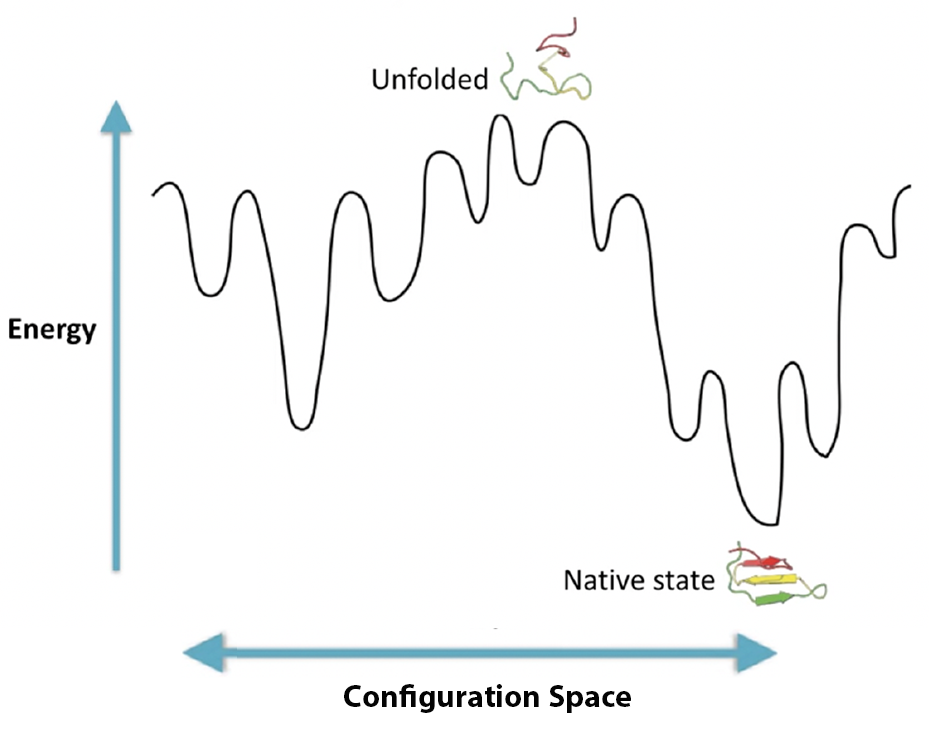
\includegraphics[width=\textwidth]{introduction/energy_landscape.png}
    \caption{Energy landscape.}
    \label{fig:landscape}
    \small
\end{figure}

To model all proteins coded by the human genome would require identifying the lowest energy structure for each of the fixed amino acids sequences for the 20 000 different proteins \cite{ponomarenko2016size}.  The protein folding research problem has been challenging for a number of reasons.  Firstly, a polypeptide chain can have a large number of different conformations; for each side chain in an amino acid in a protein there are a number of rotatable bonds with each amino acid having three different conformations leading to 3\textsuperscript{Nres} (Nres being the number of residues) possible conformations of every protein (Figure \ref{fig:angles_aa}).  Although the omega bond (peptide bond between the carbonyl carbon (C=O) of one amino acid and the nitrogen (N-H) of the adjacent amino acid in the peptide chain) is different as it is not really rotatable and results in the cis and trans forms \cite{craveur2013cis}.

\begin{figure}[th!]
    \centering
    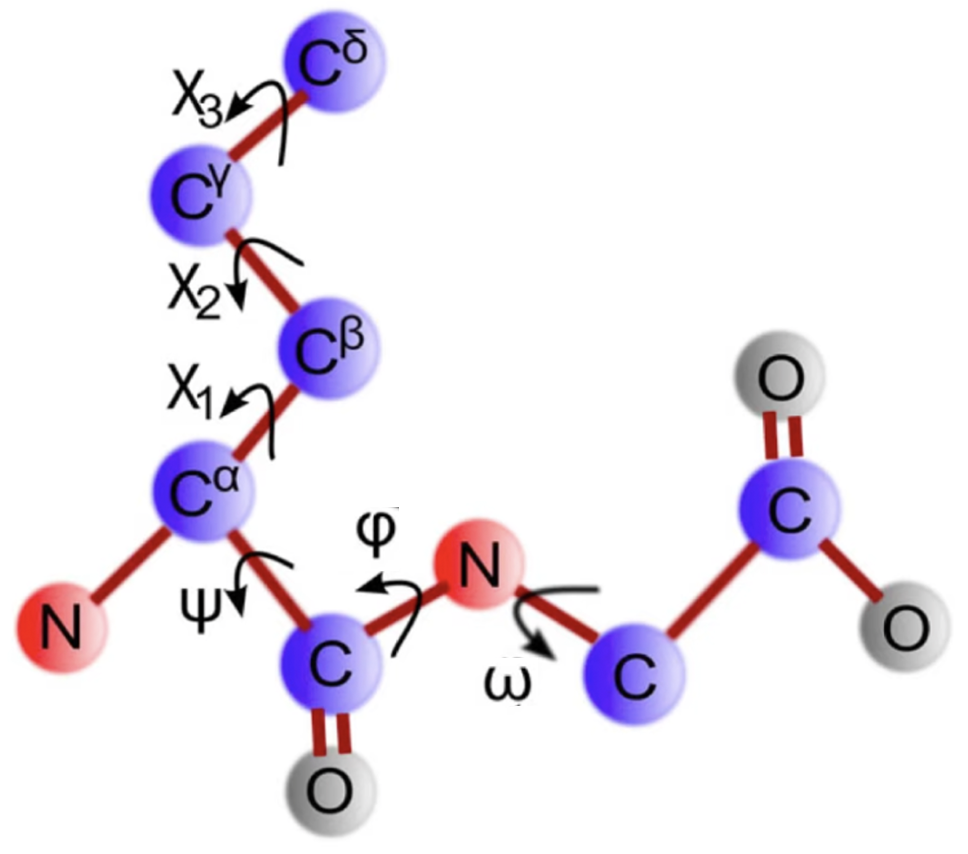
\includegraphics[width=\textwidth]{introduction/angles.png}
    \caption{Side-chain conformations.}
    \label{fig:angles_aa}
    \small
\end{figure}

Calculating the energy profile of a target protein was traditionally performed by searching through possible polypeptide chain conformations for a fixed sequence in an analogous way to how a protein naturally folds. For example Rosetta \cite{baker2001protein} simulates the actual process of folding to find the lowest energy structure rather than sampling all possible conformations.  The Rosetta folding takes place many times constructing 'decoys' to build an energy landscape to identify the lowest energy structure and therefore the most native-like structures. The folding algorithm utilises the fact that in some organisms separate genes encode interacting proteins, whereas in other organisms, their orthologues take the form of a single polypeptide chain \cite{hardin2002ab}. Therefore the structure of the protein can be viewed as a number of fragments that interact with specific kinetic and thermodynamic constraints.  During the ab initio folding process a Monte-Carlo search assembles these fragments with each assembly being scored based on a knowledge-based scoring function derived from the kinetic and thermodynamic constraints.  The model needs to capture detailed interactions between atoms therefore terms in the physics-based energy functions use mathematical means of modeling molecular interactions which need to favour:
\begin{itemize}
  \item close atomic packing (Lennard-Jones Potential \cite{jones1924determination});
  \item implicit solvation penalising buried polar atoms away from water;
  \item favour the formation of hydrogen bond interactions between polar atoms;
  \item model electrostatic interactions with the favourability of positive and negative charges to be close;
  \item model bending/torsional preferences of the polypeptide chain.
\end{itemize}
The calculation of an energy estimate or scoring function also takes the form of a knowledge-based function where statistical models define the properties of the native-like conformation. 

The method described greatly reduces the conformational search space.  However, additional strategies have also been employed to further reduce this search space.  Specifically for membrane proteins the Rosetta method was modified into a specific flavour, RosettaMembrane, where the energy function was modified to include terms that describe the interaction between target protein and the environment consisting of the anisotropic membrane. The membrane is modelled implicitly  with the energy terms including the scoring function that penalises non-helical torsion angles and non-spanning transmembrane helices within the membrane \cite{barth2007toward}.  



\section{Contact restraints used for Structure Prediction}
Contact-based modelling methods can address larger targets than conventional fragment-assembly-based ab initio methods \cite{Yang2020}. Contact-based modelling methods have been proven successful previously in modelling membrane proteins \cite{Hopf2012}.  Contact based restraints are determined by the introduction of co-variance data which supplies the additional restraints for the model building process by inferring residue-residue contacts.  The utilisation of contact predictions allows the generation of accurate ab initio models by guiding the folding process \cite{marks2011protein} .  This method led to the computational protein structure prediction for larger targets compared to what a solely fragment-assembly-based ab initio methods could construct \cite{Yang2020}. Additionally, contact-assisted ab initio modelling disposed of the need for membrane specialised folding methods like RosettaMembrane as these modelling methods have been proven successful previously in modelling membrane proteins \cite{Hopf2012,hopf2012three}.
Ab initio methods made significant strides when contact predictions were made available as modelling restraints \cite{Lee2016}. The definition of a contact is when the C$\beta$'s (C$\alpha$ in glycine) of two residues in three dimensional space are less than 8{\AA} apart.  For modelling purposes these binary contacts can be converted to distances, derived from experimental data, imposing further restraints on the modelling process \cite{braun2015combining}.   Prediction of residue-residue contacts relies on the fact that each pair of contacting residues co-varies during evolution. The process of co-variation occurs as the properties of the two residues complement each other in order to maintain structural integrity of that local region and, consequently, its original functionality (Figure \ref{fig:contacts}).  Therefore, if one residue from the pair is replaced, the other must also change to compensate the variation and hence preserve the original structure \cite{Lapedes}.  
\begin{figure}[th!]
    \centering
    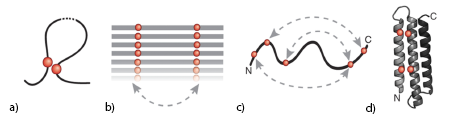
\includegraphics[width=\textwidth]{introduction/contacts.png}
    \caption{How residues separate in two-dimensions come together in three-dimensional space. }
    \label{fig:contacts}
    \small
    Interacting residues in a 3D structure compared to positions in a MSA displaying a co-evolving relationship. Adapted from \cite{Simkovic2017}.
    Co-evolutionary analysis used to infer contacts between amino acids in a protein by analysing the patterns of correlated mutations across a set of related protein sequences. a) The underlying assumption is that amino acids in close proximity within the protein structure tend to co-evolve due to their functional or structural interactions. b) Sequence Alignment: A multiple sequence alignment (MSA) is generated, which represents the amino acid sequences of related proteins. The MSA provides a basis for identifying patterns of conservation and variation across the protein family. c) based on the identified pairs of co-evolving positions, contact predictions are made, suggesting that these positions are likely in physical proximity within the protein structure. d) The inferred contacts can be visualised as a contact map or used to guide the modeling of the protein's three-dimensional structure.
\end{figure}

Initially contact prediction accuracy was limited due to transitive correlations where indirect covariation leads to a false positive contact generating noise in the prediction.  However, algorithms were developed where the link between two residues can be then reliably be detected in multiple sequence alignments. Methods included using a maximum entropy approach like direct coupling analysis (DCA) \cite{Morcos2011} or building a precision matrix (inverse co-variance matrix) like in contact prediction software PSICOV \cite{jones2012psicov}.  Early success with contact-assisted ab initio modelling of membrane proteins was made with EVfold and made use of the DCA approach in conjuction with Crystallography and NMR System (CNS) \cite{brunger1998crystallography}.  The use of contacts in this case led to substantial improvements in model accuracy for membrane proteins up to 360 residues in length and achieving RMSDs below 5{\AA} \cite{Hopf2012}.
Additionally,  machine learning algorithms were developed to predict contacts \cite{Wu2020} which was first observed in CONSIP2 \cite{kosciolek2016accurate} where evolutionary conservation was coupled with a traditional neural network with a sliding window approach. Later more advanced methods like RaptorX \cite{wang2018analysis} utilised a deep learning convoluted neural network (CNN).  CNNs are specifically designed to automatically extract hierarchical representations of input data by utilising convolutional layers, pooling layers, and fully connected layers \cite{albawi2017understanding}.  The latest methods such as TripletRes \cite{li2021deducing} exploit deep residual neural networks. Deep residual neural networks (ResNets) are a type of deep learning architecture that address the challenges of training very deep neural networks \cite{li2016demystifying}. Traditional deep neural networks suffer from the problem of vanishing gradients (where gradients are the rate of change of a function), where the gradients become very small as they propagate through many layers, leading to difficulties in training. ResNets alleviate this problem by skipping one or more layers, allowing the gradients to flow directly to the earlier layers during the training process \cite{li2016demystifying}. 

The predicted contacts can also be used for a range of analyses such as the identification of domain boundaries by analysing contact density profiles \cite{Rigden2002,Simkovic2017} and as a quality measure for ab initio models \cite{DeOliveira2016}.  Contacts can also be plotted into a two-dimensional contact map \cite{Simkovic2017} and be supplemented with other data, such as secondary structure prediction, for annotation \cite{sanchez2021conplot}.

Recent advances in contact predictions have meant more information can be extracted from MSAs allowing the prediction of residue distances rather than binary contacts.  The resultant distogram reveals more specific information in regard to predicted distances between residues in a target protein (Figure \ref{fig:distogram}). The prediction of inter-residue distances has dramatically improved the accuracy of ab initio modelling by imposing more restraints for the folding process \cite{du2021trrosetta}.  Initial attempts to go beyond binary contact prediction and predict residue distances was difficult. Methods were developed that attempted the use of regression to infer residue distances as they are real value features and therefore intuitive.  Advances were made in distance predictions when the problem was tackled as a classification problem and rather than inferring distances in {\AA} a set of bins for discrete distance values works much better with accuracy on par with contact predictions \cite{Greener2019}.

\begin{figure}[htb]
\begin{subfigure}{0.5\textwidth}
  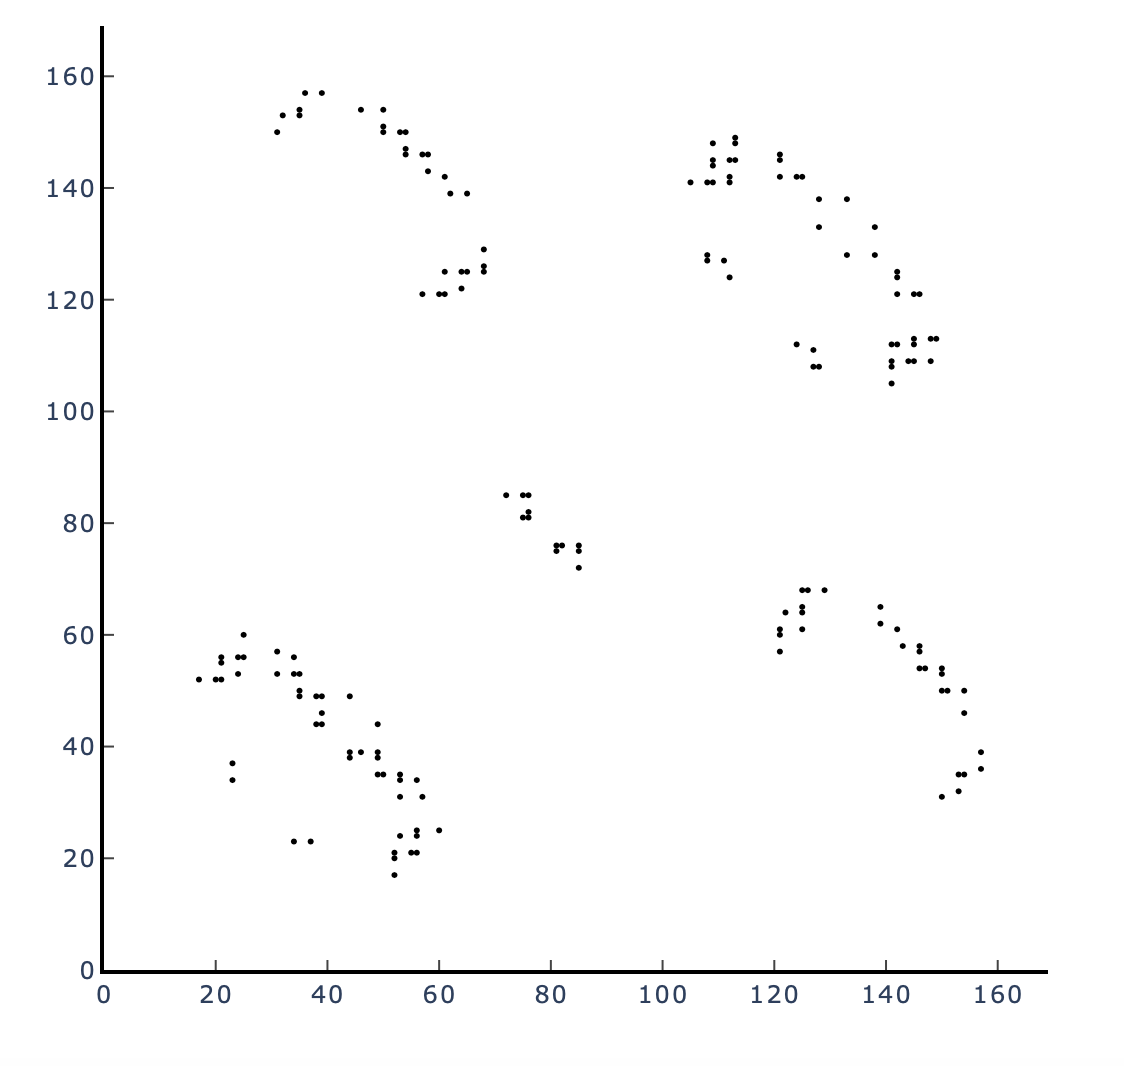
\includegraphics[width=\linewidth]{introduction/contact_map.png}
  \caption{Example contact map}
  \label{fig:4yms}
\end{subfigure}\hfil % <-- added
\begin{subfigure}{0.55\textwidth}
  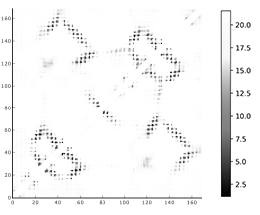
\includegraphics[width=\linewidth]{introduction/distogram.png}
  \caption{Example distogram}
  \label{fig:5do7}
\end{subfigure}\hfil % <-- added
\caption{Contact map and distogram comparison}
\small{Contacts are coloured black in the contact map; in a distogram each inter-residue pain is coloured based on a spectrum relating to the predicted distance of each specific pair of residues (in this case white to black)}
\label{fig:distogram}
\end{figure}


\section{Use of Deep Learning Algorithms for Membrane Protein Structure Prediction}
Classical protein structure prediction aimed, given a sequence, to search for the three-dimensional fold that dominates the partition function (statistical likelihood) and has the lowest free energy, making it the state most observed in nature.  The prediction of protein structure therefore possessed the twin core challenges of conformation search, ruled by Levanthal's paradox (identifying a protein's native fold by searching randomly takes an enormous amount of time yet a protein folds in seconds), and the scoring challenge, adhering to Anfinsen's dogma (the three-dimensional fold is determined by the amino acid sequence).   The well established fragment assembly ab initio approaches described in the previous section build protein models by utilising a function that models the postulates and theory derived from experimental data.  The fragment assembly methods, however, consume a high amount of computing resources and have the drawback of requiring native-like fragments being available. These methods, even with the inclusion of contact derived restraints, were only able to output reliable models for a tiny fraction of the protein universe and were especially poor for those with contact dense topologies \cite{leman2020macromolecular}.  Converting the contact information into predicted distance geometry constraints, similar to what is performed in NMR structure determination, is computationally cheaper and has been shown to produce models that are closer to their native state \cite{havel1991evaluation}.  Recently, methods such as AlphaFold, AlphaFold2 and RosettaFold have developed machine learning algorithms that predict distances which are used to generate accurate models by generating minimised free energy surface along the molecular coordinates (family-specific potentials of mean force).  The machine learning methods, or deep learning if the number of neural network layers are greater than six, construct a function to build a model by extracting features from an input data set and linking these to labels of the output data set.  Training the program involves it going back and forth in an automated fashion, taking the outputs and comparing to the inputs until a link between output and input is established.  This is similar to the classical approach where experimental data was used to construct functions that make predictions, and if the prediction were not accurate more data is gathered to refine the rules of the function; a very laborious and time consuming process.  With machine learning the function is built much more quickly with the experimental data not being used explicitly but  inferred through the learning that has taken place by linking the input features of models in the PDB (sequence) to the labels of the output structures (for example inter residue distances, main chain hydrogen bond network and torsion angles)(Figure \ref{fig:model_building}).
\begin{figure}[th!]
    \centering
    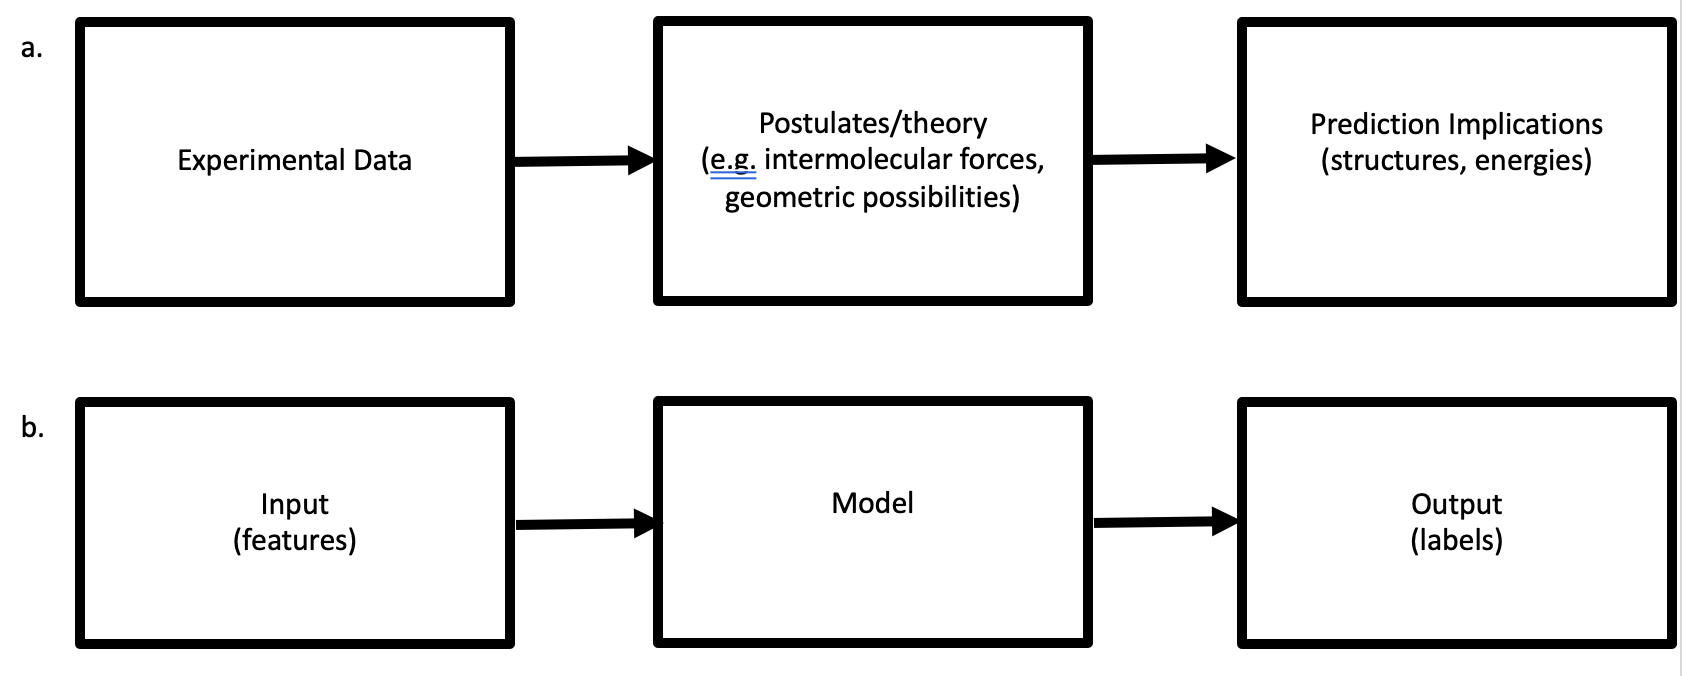
\includegraphics[width=\textwidth]{introduction/model_building.png}
    \caption{Comparison of the model function building between classical (a) and machine learning (b) methods}
    \label{fig:model_building}
    \small
\end{figure}

The deep learning methods such as AlphaFold \cite{Jumper2021}, DMPfold \cite{Greener2019} and trRosetta \cite{yan2021accurate} build predicted protein structures by predicting inter residue distances, main chain hydrogen bond network and torsion angles.  Benchmarking these methods has demonstrated that they work just as well for membrane proteins as they do for soluble proteins \cite{Greener2019,hegedHus2021alphafold2}.  DMPfold was shown to be able to model 26 of the 28 transmembrane proteins with a TM-score of at least 0.5 to the native structure and a mean TM-score of 0.74 \cite{Greener2019}.  The accuracy of AlphaFold2 transmembrane protein modeling has been tested by exploring the construction of structures from the ABC protein superfamily. For these transmembrane proteins AlphaFold2 performed exceedingly well when testing template-free structure prediction as well as attempting a new ABC fold, dimer modeling, and stability in molecular dynamics simulations \cite{hegedHus2021alphafold2}.  

\section{Exploitation of Advanced Methods}
This thesis details the utilisation of the methods described to build models of three intracellular organelle residing integral membrane proteins.  Unusual structural features are predicted during the investigation and subsequently methods for screening membrane proteins possessing these features were implemented. The work carried out during this PhD intersects with the unexpected acceleration in the field of protein structure prediction initiated in CASP13 with the release of AlphaFold \cite{Jumper2021}. The release of the accurate deep learning protein structural prediction methods half way through the PhD gave the opportunity to modify research plans in order to take advantage of these fast and accurate methods.  For example, in Chapter 3, a topology was mapped for the protein Tmem41b using contact map analysis; with the release of DMPfold, an accurate three dimensional model could be constructed which displayed the re-entrant loops that fragment assembly methods could not build.  Furthermore, the release of the AlphaFold database \cite{david2022alphafold} enabled a library of trRosetta models to be enriched with the more accurate AlphaFold equivalents; this enabled us to search for specific structural motifs within a library of high quality models that had no experimental structures (Chapter 5).  The field of protein structure is currently moving at a very fast pace and I feel privileged to have been in this field, as a researcher utilising these bioinformatic methods as well as my role as a CASP assessor in CASP14, at this very important juncture.   
